\documentclass[12pt]{standalone}

\usepackage{xcolor}
\usepackage[prefix=solar-]{xcolor-solarized}

\usepackage{tikz}

\begin{document}
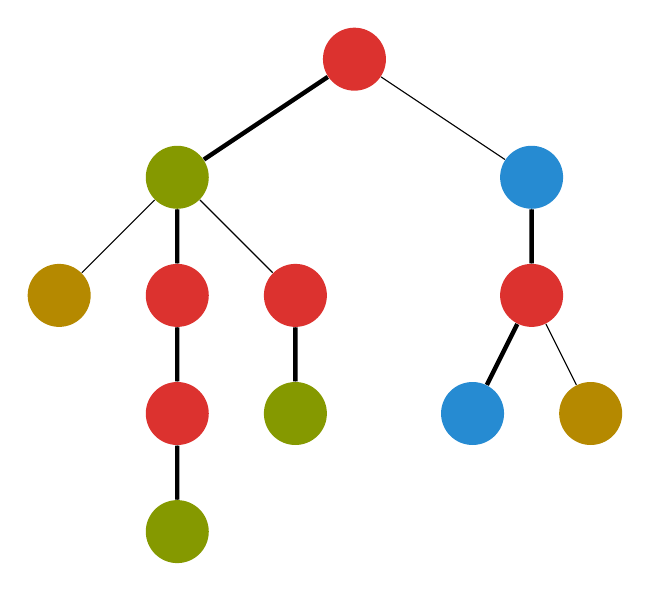
\begin{tikzpicture}[x=15mm,y=15mm]
    \begin{scope}[every node/.style={circle,fill,minimum size=8mm}]
        \node[solar-red] (A) at (0,1) {};

        \node[solar-green] (B) at (-1.5,0) {}
            child {node[solar-yellow] (C) {}}
            child {node[solar-red] (D) {}
                child {node[solar-red] (E) {}
                    child {node[solar-green] (F) {}}}}
            child {node[solar-red] (G) {}
                child {node[solar-green] (H) {}}};

        \node[solar-blue] (I) at (1.5,0) {}
            child {node[solar-red] (J) {}
                child {node[solar-blue] (K) {}}
                child {node[solar-yellow] (L) {}}};
    \end{scope}

    \path (A) edge (B) edge (I);

    \path[ultra thick]
        (A) edge (B)
        (B) edge (D)
        (D) edge (E)
        (E) edge (F)
        (G) edge (H)
        (I) edge (J)
        (J) edge (K);
\end{tikzpicture}
\end{document}
